\chapter{La presión del aire y el tiempo atmosférico}\label{ch:g5:air-pressure-weather}

Vives en el fondo de un océano --- un océano de \omterm{def:g2:air-around-us:air}{aire}, de cientos de
kilómetros de profundidad, con todo su \omterm{def:g4:weight-and-mass:weight}{peso} descansando sobre tus
hombros. ¿Por qué no te aplasta? ¿Por qué ni siquiera lo notas? ¿Y qué
tiene que ver todo esto con el tiempo que hará mañana? El \omterm{def:g2:air-around-us:air}{aire},
nuestro viejo amigo invisible, tiene todavía un secreto grande que
entregar.

\section{El aire pesa}

\begin{example}[Pesar lo invisible]\label{ex:g5:air-pressure-weather:weighing}
Se coloca un balón bien hinchado en una \omterm{def:g3:levers-and-scales:scale}{balanza} fina y se equilibra
exactamente. Después se abre su válvula y el \omterm{def:g2:air-around-us:air}{aire} de más sale
silbando --- el mismo balón, la misma válvula, todo igual, menos un
poco de \omterm{def:g2:air-around-us:air}{aire}. De vuelta a la \omterm{def:g3:levers-and-scales:scale}{balanza}: el balón deshinchado es
\emph{más ligero}. La diferencia es el \omterm{def:g4:weight-and-mass:weight}{peso} del \omterm{def:g2:air-around-us:air}{aire} que se ha
escapado. El \omterm{def:g2:air-around-us:air}{aire} es materia, la materia tiene \omterm{def:g3:measuring-mass:mass}{masa} y de la
\omterm{def:g3:measuring-mass:mass}{masa} tira la Tierra hacia abajo: el océano que tenemos encima pesa.
\end{example}

\begin{definition}[La atmósfera y su presión]\label{def:g5:air-pressure-weather:pressure}
La \emph{atmósfera}\index{atmósfera} es la capa profunda de \omterm{def:g2:air-around-us:air}{aire}
que envuelve la Tierra entera. Su \omterm{def:g4:weight-and-mass:weight}{peso} aprieta el \omterm{def:g2:air-around-us:air}{aire} del fondo
--- donde vivimos ---, y el \omterm{def:g2:air-around-us:air}{aire} apretado empuja con fuerza sobre
todas las superficies que toca. A ese empuje se le llama \emph{presión
atmosférica}\index{presión atmosférica}.
\end{definition}

\begin{proposition}[El empuje por todos lados]\label{prop:g5:air-pressure-weather:allsides}
La \omterm{def:g5:air-pressure-weather:pressure}{presión atmosférica} empuja sobre todas las superficies desde
\emph{todas} las direcciones --- hacia abajo sobre las mesas, de lado
sobre las paredes e incluso \emph{hacia arriba} sobre los techos y las
palmas de las manos. Y es tremenda: sobre una superficie del tamaño de
tu palma, el \omterm{def:g2:air-around-us:air}{aire} empuja más o menos con el \omterm{def:g4:weight-and-mass:weight}{peso} de una maleta
grande y llena. No nos enteramos nunca porque los empujes llegan
equilibrados: el \omterm{def:g2:air-around-us:air}{aire} que hay dentro de nosotros y detrás de cada
superficie empuja de vuelta con la misma \omterm{def:g2:pushes-and-pulls:force}{fuerza}.
\end{proposition}

\begin{method}[La cartulina que sujeta el agua]\label{met:g5:air-pressure-weather:card}
El empuje hacia arriba del \omterm{def:g2:air-around-us:air}{aire}, pillado con las manos en la \omterm{def:g3:measuring-mass:mass}{masa}
(hazlo sobre el fregadero):
\begin{enumerate}
  \item llena un vaso de agua hasta el borde mismo;
  \item pon encima, plana, una cartulina rígida y lisa que toque el
        agua por todo el contorno;
  \item sujeta la cartulina en su sitio, dale la vuelta al vaso
        exactamente boca abajo y suelta la cartulina con suavidad.
\end{enumerate}
La cartulina se queda --- sujetando el vaso lleno entero. El \omterm{def:g4:weight-and-mass:weight}{peso}
del agua aprieta la cartulina hacia abajo, pero la \omterm{def:g5:air-pressure-weather:pressure}{atmósfera} la
aprieta \emph{hacia arriba} con todavía más \omterm{def:g2:pushes-and-pulls:force}{fuerza}. Acabas de ver el
empuje de la maleta desde abajo.
\end{method}

\begin{omfigure}
\begin{tikzpicture}[scale=0.85]
  \draw[thick] (4.4,1.2) -- (4.4,3.6) (6.6,1.2) -- (6.6,3.6);
  \draw[thick] (4.4,3.6) -- (6.6,3.6);
  \fill[omDef, opacity=0.25] (4.4,1.25) rectangle (6.6,3.55);
  \draw[very thick, omMeth] (4.25,1.2) -- (6.75,1.2);
  \node[right, font=\small, omMeth] at (6.9,1.2) {la cartulina};
  \draw[-Stealth, thick, omDef] (5.0,2.9) -- (5.0,2.2);
  \draw[-Stealth, thick, omDef] (6.0,2.9) -- (6.0,2.2);
  \node[above, font=\small, omDef] at (5.5,3.65)
    {el agua empuja hacia abajo};
  \foreach \x in {4.7,5.5,6.3} {
    \draw[-Stealth, very thick, omThm] (\x,0.15) -- (\x,0.95);
  }
  \node[below, font=\small, omThm] at (5.5,-0.05)
    {la atmósfera empuja hacia arriba --- con más fuerza};
\end{tikzpicture}

{\small El vaso boca abajo: el empuje del \omterm{def:g2:air-around-us:air}{aire} hacia arriba sobre la
cartulina puede más que el \omterm{def:g4:weight-and-mass:weight}{peso} del agua. El océano invisible es
fuerte.}
\end{omfigure}

\section{Máquinas movidas por la atmósfera}

\begin{example}[La pajita]\label{ex:g5:air-pressure-weather:straw}
Crees que subes el zumo tirando de él por la pajita. En realidad, un
\omterm{def:g3:solids-liquids-gases:liquid}{líquido} no se puede estirar --- ¡prueba a tirar del agua con los
dedos! Lo que haces de verdad es sorber el \emph{\omterm{def:g2:air-around-us:air}{aire}} que hay dentro
de la pajita. Sin \omterm{def:g2:air-around-us:air}{aire} dentro, la \omterm{def:g5:air-pressure-weather:pressure}{atmósfera} que aprieta el zumo
del vaso empuja el zumo pajita arriba hasta tu boca. Cada sorbo es la
\omterm{def:g5:air-pressure-weather:pressure}{atmósfera} haciendo el levantamiento; tú solo despejas la carretera.
\end{example}

\begin{example}[Ventosas y botellas aplastadas]\label{ex:g5:air-pressure-weather:suction}
La ventosa de goma del colgador del baño se aprieta contra los azulejos
y expulsa el \omterm{def:g2:air-around-us:air}{aire} de debajo: ahora la \omterm{def:g5:air-pressure-weather:pressure}{atmósfera} aprieta la ventosa
contra la pared sin que nada empuje de vuelta por detrás --- clavada
por el propio cielo. Y enrosca el tapón de una botella de plástico
vacía en lo alto de una montaña y baja después en coche hasta el valle:
la botella se arruga como si la estrujara una mano fantasma. Fuera
aprieta más \omterm{def:g2:air-around-us:air}{aire} que el \omterm{def:g2:air-around-us:air}{aire} enrarecido de montaña que quedó
encerrado dentro --- gana la \omterm{def:g5:air-pressure-weather:pressure}{atmósfera} y la botella se pliega.
\end{example}

\begin{example}[Más enrarecido con la altura]\label{ex:g5:air-pressure-weather:height}
Sube y dejarás parte del océano por debajo de ti: menos \omterm{def:g2:air-around-us:air}{aire} encima
significa un empuje más débil. Los oídos se te destaponan en un
teleférico rápido, según cambia la presión de fuera; los montañeros
jadean en un \omterm{def:g2:air-around-us:air}{aire} enrarecido. Y aquí se rinde el misterio del té de
montaña del año pasado: si la \omterm{def:g5:air-pressure-weather:pressure}{atmósfera} aprieta menos el agua,
hervir resulta más fácil --- en las grandes cumbres el agua hierve
bastante por debajo de \qty{100}{\celsius}, demasiado fría para hacer
un té como es debido.
\end{example}

\begin{omfigure}
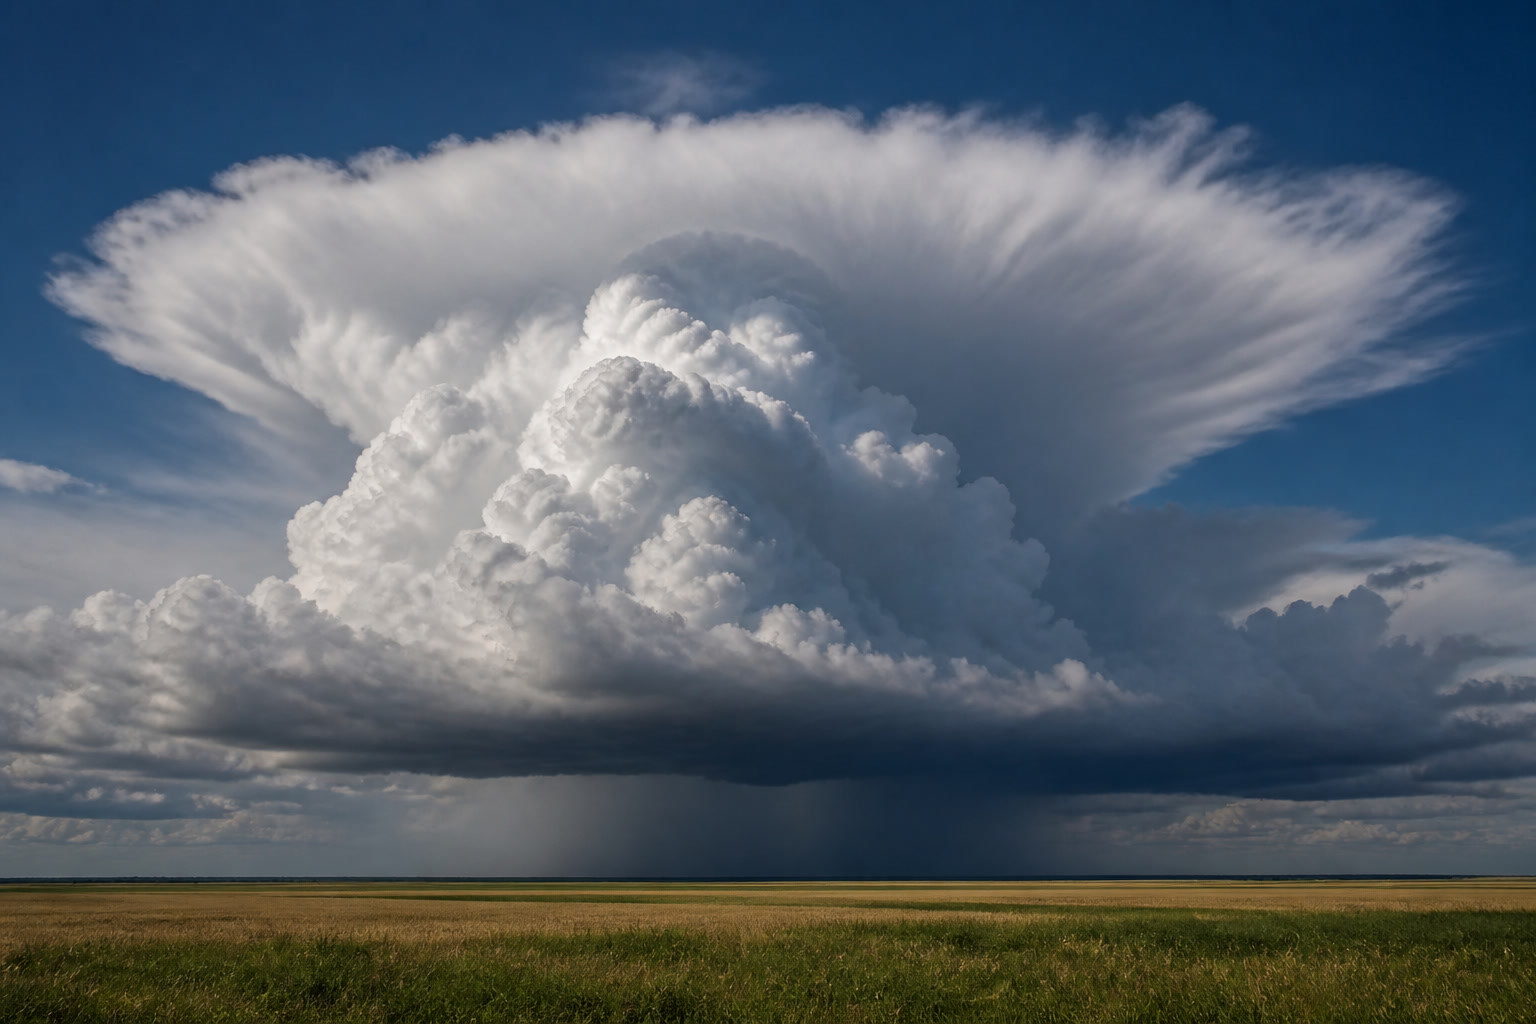
\includegraphics[width=0.58\linewidth]{images/book1/ai/g5-weather-storm.jpg}

{\small Una nube de tormenta creciendo sobre los campos: el tiempo atmosférico es la \omterm{def:g5:air-pressure-weather:pressure}{atmósfera} en movimiento.}
\end{omfigure}

\section{El barómetro y el tiempo}

\begin{definition}[Barómetro]\label{def:g5:air-pressure-weather:barometer}
Un \emph{barómetro}\index{barómetro} es el instrumento que mide la
\omterm{def:g5:air-pressure-weather:pressure}{presión atmosférica} --- un miembro más de nuestra familia de jueces
honrados, junto al \omterm{def:g3:temperature-thermometers:temperature}{termómetro} y a la \omterm{def:g3:levers-and-scales:scale}{balanza}. Su aguja sube cuando
la \omterm{def:g5:air-pressure-weather:pressure}{atmósfera} de arriba aprieta más fuerte y baja cuando el apretón
se afloja.
\end{definition}

\begin{proposition}[La presión habla del mañana]\label{prop:g5:air-pressure-weather:weather}
La presión de la \omterm{def:g5:air-pressure-weather:pressure}{atmósfera} es inquieta: el \omterm{def:g2:air-around-us:air}{aire} pesado que baja
trae cielos tranquilos y despejados; el \omterm{def:g2:air-around-us:air}{aire} ligero que sube
invita a las nubes y a la lluvia. Así que el \omterm{def:g5:air-pressure-weather:barometer}{barómetro} es un
adivino modesto y honrado: una presión \emph{estable o en subida}
promete buen tiempo; una presión \emph{en bajada} avisa de que vienen
nubes; y una \emph{bajada rápida} significa que puede haber tormenta
en camino.
\end{proposition}

\begin{omfigure}
\begin{tikzpicture}[scale=0.85]
  \draw[thick] (2.2,1.7) circle (1.5);
  \foreach \a/\t in {150/{}, 120/{}, 90/{}, 60/{}, 30/{}} {
    \draw (2.2,1.7) ++(\a:1.3) -- ++(\a:0.18);
  }
  \node[font=\footnotesize] at (1.1,2.6) {lluvia};
  \node[font=\footnotesize] at (2.2,3.0) {variable};
  \node[font=\footnotesize] at (3.4,2.6) {buen tiempo};
  \draw[-Stealth, very thick, omThm] (2.2,1.7) -- ++(55:1.1);
  \fill (2.2,1.7) circle (2pt);
  \node[below, font=\small] at (2.2,-0.05)
    {un barómetro de casa: la aguja se inclina hacia el buen tiempo};
  \node[right, font=\small, align=left] at (5.4,2.5)
    {aguja en subida: cielos despejados a la vista};
  \node[right, font=\small, align=left] at (5.4,1.7)
    {aguja en bajada: se juntan las nubes};
  \node[right, font=\small, align=left] at (5.4,0.9)
    {bajada rápida: a resguardarse --- tormenta};
\end{tikzpicture}

{\small Leer un \omterm{def:g5:air-pressure-weather:barometer}{barómetro}: no importa tanto dónde está la aguja como
hacia dónde se mueve --- la \omterm{def:g5:air-pressure-weather:pressure}{atmósfera} anuncia sus planes.}
\end{omfigure}

\begin{remark}[La A y la B del mapa del tiempo]\label{rem:g5:air-pressure-weather:map}
El parte del tiempo de esta noche enseñará grandes remolinos marcados
con una A y con una B: regiones de presión alta y baja que van a la
deriva por el mapa como ballenas lentas. El \omterm{def:g2:air-around-us:air}{aire} fluye sin parar
desde las pesadas regiones de la A hacia las ligeras regiones de la
B --- y ese fluir \emph{es el \omterm{def:g2:air-around-us:wind}{viento}}. Un solo capítulo, tres viejos
amigos explicados: la predicción del \omterm{def:g5:air-pressure-weather:barometer}{barómetro}, el origen del
\omterm{def:g2:air-around-us:wind}{viento} y la razón por la que tus oídos saben cuándo va a cambiar el
tiempo.
\end{remark}

\section{Ejercicios}

\begin{exercise}[$\star$]\label{exo:g5:air-pressure-weather:1}
¿Cómo demuestra el experimento del balón que el \omterm{def:g2:air-around-us:air}{aire} tiene
\omterm{def:g4:weight-and-mass:weight}{peso}? ¿Qué es exactamente lo que se compara?
\end{exercise}

\begin{exercise}[$\star$]\label{exo:g5:air-pressure-weather:2}
¿Qué es la \omterm{def:g5:air-pressure-weather:pressure}{presión atmosférica} y de dónde viene? ¿En qué direcciones
empuja?
\end{exercise}

\begin{exercise}[$\star$]\label{exo:g5:air-pressure-weather:3}
La \omterm{def:g5:air-pressure-weather:pressure}{atmósfera} aprieta la palma de tu mano más o menos con lo que
pesa una maleta llena --- y sin embargo no notas nada. ¿Por qué no?
\end{exercise}

\begin{exercise}[$\star$]\label{exo:g5:air-pressure-weather:4}
En el truco de la cartulina, dos empujes se pelean por ella.
Nómbralos y di cuál gana.
\end{exercise}

\begin{exercise}[$\star$]\label{exo:g5:air-pressure-weather:5}
``Subo el zumo tirando de él por la pajita''. Corrige esta frase: ¿qué
es lo que quitas de verdad y quién hace el levantamiento?
\end{exercise}

\begin{exercise}[$\star$]\label{exo:g5:air-pressure-weather:6}
¿Por qué se agarra una ventosa a los azulejos? ¿Qué se ha expulsado y
qué es lo que sujeta la ventosa?
\end{exercise}

\begin{exercise}[$\star$]\label{exo:g5:air-pressure-weather:7}
¿Qué le pasa a la \omterm{def:g5:air-pressure-weather:pressure}{presión atmosférica} cuando subes una montaña y por
qué? Da dos señales de ello que pueda notar un viajero.
\end{exercise}

\begin{exercise}[$\star$]\label{exo:g5:air-pressure-weather:8}
¿Qué mide un \omterm{def:g5:air-pressure-weather:barometer}{barómetro}? Tu \omterm{def:g5:air-pressure-weather:barometer}{barómetro} lleva bajando deprisa
desde el desayuno --- ¿qué le espera al plan del picnic?
\end{exercise}

\begin{exercise}[$\star\star$]\label{exo:g5:air-pressure-weather:9}
La botella cerrada se arrugó durante la bajada de la montaña. Explica
el arrugamiento con los empujes de dentro y de fuera --- y predice:
¿qué le pasaría en cambio a una botella cerrada en el valle y llevada
\emph{hacia arriba}?
\end{exercise}

\begin{exercise}[$\star\star$]\label{exo:g5:air-pressure-weather:10}
¿De dónde viene el \omterm{def:g2:air-around-us:wind}{viento}, según los remolinos de la A y la B del
mapa del tiempo? Conéctalo con la definición más antigua de este
libro: el \omterm{def:g2:air-around-us:wind}{viento} es \omterm{def:g2:air-around-us:air}{aire} en movimiento --- ¿movido por qué?
\end{exercise}

\begin{exercise}[$\star\star$]\label{exo:g5:air-pressure-weather:11}
Los alpinistas se quejan de que en las grandes cumbres el té nunca
sale fuerte y la pasta se queda dura por mucho que hierva. Reúne la
explicación completa a lo largo de dos años: ¿qué le hace la
\omterm{def:g5:air-pressure-weather:pressure}{atmósfera} enrarecida al \omterm{def:g4:changes-of-state:boiling-point}{punto de ebullición} y por qué no sirve
de nada hervir más rato? (Dos proposiciones, una de ellas del año
pasado, cierran el caso.)
\end{exercise}
